\documentclass[	DIV=calc,%
							paper=a4,%
							fontsize=11pt,%
							twocolumn]{scrartcl}	 					% KOMA-article class

\usepackage{lipsum}													% Package to create dummy text
\usepackage[english]{babel}										% English language/hyphenation
\usepackage[protrusion=true,expansion=true]{microtype}				% Better typography
\usepackage{amsmath,amsfonts,amsthm}					% Math packages
\usepackage[pdftex]{graphicx}									% Enable pdflatex
\usepackage[svgnames]{xcolor}									% Enabling colors by their 'svgnames'
\usepackage[hang, small,labelfont=bf,up,textfont=it,up]{caption}	% Custom captions under/above floats
\usepackage{epstopdf}												% Converts .eps to .pdf
\usepackage{subfig}													% Subfigures
\usepackage{booktabs}												% Nicer tables
\usepackage{fix-cm}	
\usepackage{color}
\usepackage{hyperref}
\usepackage{amsmath}
\usepackage{amssymb}
\usepackage{tikz}
\usepackage{tabularx}
\usepackage{amsmath}
\usepackage{layouts}
\usepackage{array}
\usepackage{tikz}
\usepackage{amssymb}
\usepackage{graphics}
\usepackage{lmodern}
\usepackage{epstopdf}
\usepackage[T1]{fontenc}
\usepackage[utf8]{inputenc}
\usepackage{authblk}
\usepackage{tabularx}
\usepackage{multirow}
\usepackage{bm}
\usepackage{here}
\usepackage{biblatex} 
\bibliography{report} 
\usepackage{enumerate}
\usepackage{booktabs}	
\usepackage{algorithm}
\usepackage{algorithmic}


%%% Custom sectioning (sectsty package)
\usepackage{sectsty}													% Custom sectioning (see below)
\allsectionsfont{%															% Change font of al section commands
	\usefont{OT1}{phv}{b}{n}%										% bch-b-n: CharterBT-Bold font
	}

\sectionfont{%																% Change font of \section command
	\usefont{OT1}{phv}{b}{n}%										% bch-b-n: CharterBT-Bold font
	}


\hypersetup{
  colorlinks,%
    citecolor=black,%
    filecolor=black,%
    linkcolor=black,%
    urlcolor=black
}

%%% Headers and footers
\usepackage{fancyhdr}												% Needed to define custom headers/footers
	\pagestyle{fancy}														% Enabling the custom headers/footers
\usepackage{lastpage}	

% Header (empty)
\lhead{}
\chead{}
\rhead{}
% Footer (you may change this to your own needs)
\lfoot{\footnotesize \texttt{NAO Localization} \textbullet ~University of Amsterdam}
\cfoot{}
\rfoot{\footnotesize page \thepage\ of \pageref{LastPage}}	% "Page 1 of 2"
\renewcommand{\headrulewidth}{0.0pt}
\renewcommand{\footrulewidth}{0.4pt}



%%% Creating an initial of the very first character of the content
\usepackage{lettrine}
\newcommand{\initial}[1]{%
     \lettrine[lines=3,lhang=0.3,nindent=0em]{
     				\color{DarkGoldenrod}
     				{\textsf{#1}}}{}}



%%% Title, author and date metadata
\usepackage{titling}															% For custom titles

\newcommand{\HorRule}{\color{DarkGoldenrod}%			% Creating a horizontal rule
									  	\rule{\linewidth}{1pt}%
										}

\pretitle{\vspace{-30pt} \begin{flushleft} \HorRule 
				\fontsize{50}{50} \usefont{OT1}{phv}{b}{n} \color{DarkRed} \selectfont 
				}
\title{NAO Localization}					% Title of your article goes here
\posttitle{\par\end{flushleft}\vskip 0.5em}

\preauthor{\begin{flushleft}
					\large \lineskip 0.5em \usefont{OT1}{phv}{b}{sl} \color{DarkRed}}
\author{Amogh Gudi, Georgios K. Methenitis, Nikolaas Steenbergen, Patrick de Kok\\}											% Author name goes here
\postauthor{\footnotesize \usefont{OT1}{phv}{m}{sl} \color{Black} 
					University of Amsterdam 								% Institution of author
					\par\end{flushleft}\HorRule}

\date{}																				% No date



%%% Begin document
\begin{document}
\maketitle
\thispagestyle{fancy} 			% Enabling the custom headers/footers for the first page 
% The first character should be within \initial{}
\initial{I}\textbf{n this Project we propose a basic code for the Robo soccer Standard league Platform for the Dutch national team. We focused on the problem of visual feature recognition and the localization of the robot in a tournament setup. This project contains a detailed description of our implementation together with a conclusion and a brief evaluation. Since this report only covers feature detection and Localization we give an outlook on what parts are to be implemented in addition to make the robots play soccer.}

\section{Feature Extraction}
Visual object recognition is a key ability for autonomous robotic agents especially in dynamic and partially observable environments. A reliable landmark detection process is really crucial for achieving self-localization, which can be easily considered as the stepping stone for having a functional robotic soccer team. In this section, we describe the whole procedure of processing input images from the NAO's camera, outputting features that are informative to be used by the core of our localization scheme.  Using a variety of image processing techniques, we successfully detect field landmarks. In general, we have to deal with noisy images, which not only contain the field region but also background noise and useless information which comes from above the horizon of the field view. Furthermore, we had to deal with lighting conditions which may vary significantly.
There also real-time constraints which had to be taken into consideration during our algorithmic implementation in order for the whole procedure to be able to execute in real time.

\begin{figure}[t!]
  \caption{HSV colorspace. \href{http://en.wikipedia.org/wiki/HSL_and_HSV}{( Image source )}}
  \label{hsv}
  \centering
    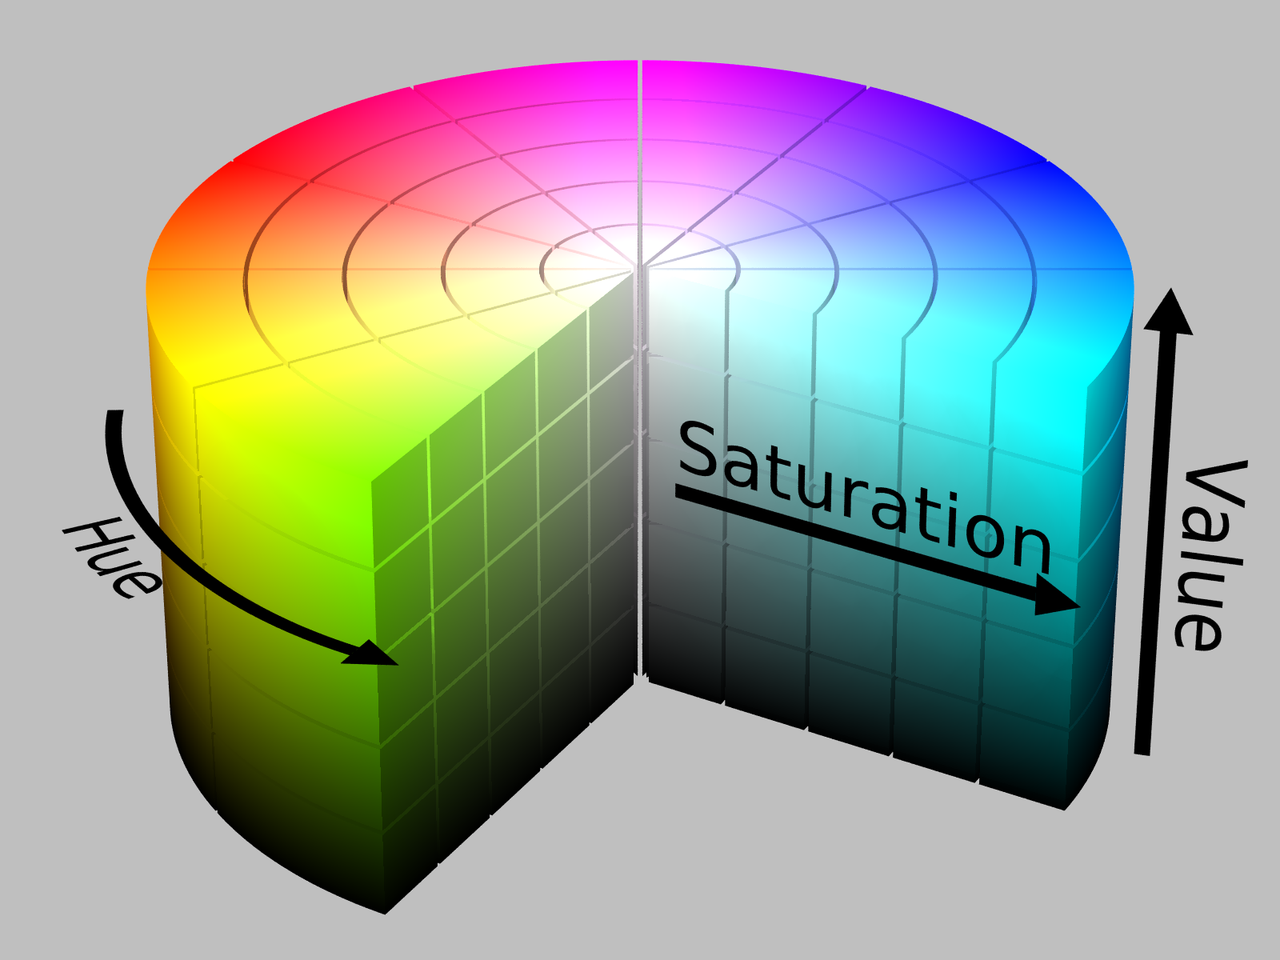
\includegraphics[width=0.3\textwidth]{figures/1280px-HSV_color_solid_cylinder_alpha_lowgamma.png}
\end{figure}

\subsection{Choosing colorspace}
The first challenge we came along was to choose the best colorspace representation in order to overcome the variations in lighting conditions. The dataset we had consisted from rgb images. Unfortunately, it was unfeasible to use the default rgb colorspace for most applications due to noise, shadows, etc. We also experimented with normalized rgb colorspace. Theoretically,  normalized rgb would have given us the pure chromaticity values of each object in our field of view, overcoming like this possible shadows and lighting conditions. In the contrary, normalized rgb did not help us achieving a light-invariant color representation, resulting into false positives in color segmentation. HSV was the solution to our problem. HSV is a cylindrical colorspace representation, which contains information about hue, saturation, and value. We found hue to be really informative in order to distinguish  easily between the colors. Hue define the pure chromaticity of the color and it is independent of the lighting conditions. In figure~\ref{hsv}, we illustrate this cylindrical color representation, we can see that the hue is represented by the angular dimension in the vertical axis of the cylinder. 


\subsection{Basic Pipeline}
Having described the first basic step of our approach, choosing the proper colorspace for our application, it is time to go deeper into the feature extraction procedure.
The first step in this procedure is the image input from the NAO's camera in HSV format. As we said before, images not only contain the important region of the field in which we are interested in, but also some background information which is useless in order to detect field features. This background usually extends above the field horizon and it may become really disturbing in the extraction process. This is the reason why background removal is the first step in our feature extraction scheme. Once we have removed, our input image contains information which has to be extracted. Field lines, goals, ball, and other NAO robots are the features located into the field. In this project, we only took into consideration lines, and the goals which are static landmarks, as ball, and other robots are moving and we cannot depend on them in order to self-localize. So, we use information from the HSV values to binarize the image, first in respect to the goals and then in respect to the lines. As we said in the introduction part of this paper, field is colored green, both goals are yellow, and lines are white. Next step of the feature extraction is the the goal detection, making use of the horizontal and vertical histograms of yellow values. Line detection is followed in order to find a good estimation about the lines detected in our field of view. Having these lines' estimations, we can detect feature on them, using geometric properties. Last step in this process' pipeline is to output all these detected features to the localization core process. We can now enumerate all steps in these pipeline, these are:
\begin{enumerate}
\item Input HSV image from camera
\item Background removal
\item Image binarization
\item Line detection
\item Line feature detection
\item Goal detection
\item Output features
\end{enumerate}



\section{Image format}
NAO's camera can output images in different colorspaces representations. The images from the dataset we had, were in RGB format, and they had QVGA resolution ($320 \times 240$). We wanted to keep a low resolution in order to keep the time complexity of our algorithm feasible for real-time execution. \textbf{Patrick can add some things here as he experimented better with NAO's camera.}

\begin{table}
\begin{center}
\caption{Threshold values used for color segmentation.}
\label{thresholdHSV}
\begin{tabular}{lccc}
\toprule
\multicolumn{4}{c}{\textbf{Threshold}} \\
\cmidrule(r){2-4}
\textbf{Color}   & \textbf{Hue} & \textbf{Saturation} & \textbf{Value} \\
\midrule
Green      & $20 \sim 37$    & $100 \sim 255$    & $100 \sim 255$    \\
Yellow      & $38 \sim 75$    & $50 \sim 255$    & $50 \sim 255$    \\
White     & $0 \sim 255$    & $0 \sim 60$    & $200 \sim 255$    \\
\bottomrule
\end{tabular}
\end{center}
\end{table}

\section{Background Removal}
Background removal defines the task of detecting the field's borders in order to exclude uninformative regions in the processing image, saving this way computational cost and helping to subtract only the useful part of the image, which is the one, where we can detect all the features we are interested in. This can be done by a vertical scan of the image and detecting the first green pixel in each column. This method can work efficiently but it is not robust in many cases, as green pixels can be found above the field's horizon as well. Following the same principle in our approach, we consider as background every region upon a column before a considerable amount of green pixels, and not just one, which can lead us to faulty decisions about the horizon. We start in each column considering the pixel in the first row as background. Then, during scanning each column, we stop when we find many green continuous pixels and assign as horizon row in this column the first of this sequence of green pixels. In this process, we are only interested in green pixels. As you can see in table~\ref{thresholdHSV}, green pixels are considered as those which have hue, saturation, and value around these thresholds. Figure~\ref{background}, illustrates the process of background removal. Even though it is not such a sophisticated method, we can see that in this specific example, almost all background above the field's horizon has been removed, helping us in this way to avoid detect false positive features in the background.

\begin{figure*}[t!]
\caption{Background removal process example, original RGB image (left), points indicating the start of the field (middle), regions of interest without background information (right).}
\label{background}
\centering    
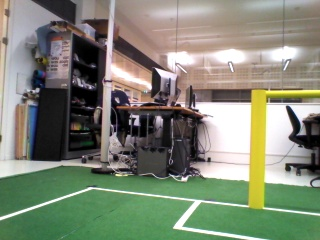
\includegraphics[width=0.3\textwidth]{figures/original.png} \	
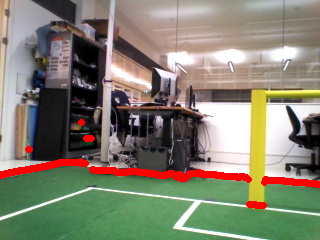
\includegraphics[width=0.3\textwidth]{figures/back.png} \	
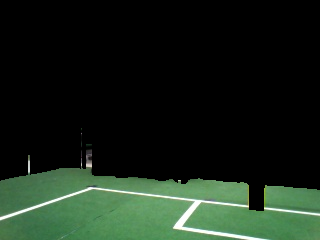
\includegraphics[width=0.3\textwidth]{figures/back_fixed.png}	
\end{figure*}


\section{Image Binarization}
In this section, we will talk about another image pre-processing technique which helped our main procedure detect features easier. Image binarization is a process which outputs two binary images, one in respect to the goals, and the other in respect to the field lines. For goal detection, it is natural that we are interested only in yellow areas of the image. The same applies for field lines, we are only interested in green and white areas of it. The main goal of this process is to classify colors according to table~\ref{thresholdHSV}. As we can realize, a simple way to classify colors is used in order to get a binary image, with the interesting part highlighted in each case. For the first case, goals, we are only interested to find yellow, so we output white for each yellow pixel, and black for any other color. For field lines, black for every other than white pixel.

\begin{figure}[h!]
\caption{Binary images in respect to the lines (left),  and to the goal (right), for the example RGB image in Figure~\ref{background}.}
\label{binary}
\centering    
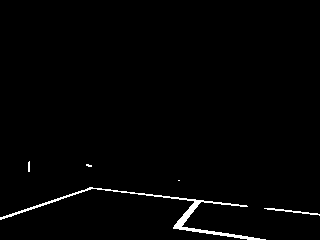
\includegraphics[width=0.22\textwidth]{figures/bin_lines.png} \	
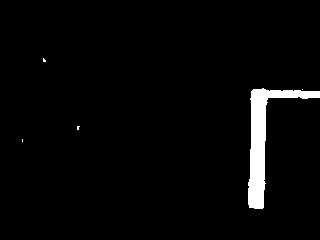
\includegraphics[width=0.22\textwidth]{figures/bin_posts.png} \	
\end{figure}

Figure~\ref{binary}, illustrates the process of image binarization. To add some technical details about the above implementation of image binarization, we can say that the whole process of it is integrated into the background removal procedure which requires only one vertical scan of the input image, and its goal is to minimize the space complexity of the whole feature extraction method as now we have only to process binary images with only one channel, in contrast to the original 3-channel image.

\section{Line Detection}
Before proceeding to the exact procedure about finding goals and line features, it is time to introduce our proposing approach to detect line segments in a binary image like those we presented before in image binarization section.

\subsection{Other approaches}
In general, we are interested in finding one line segment for each actual line segment appearing in the image. Other methods, such as Hough Transformation or Probabilistic Hough Transformation failed to detect these continuous line segments, due to the fact that they applied after edge detection step. Lines in our images consist of line segments which are thicker than one pixel, and when edge detection is applied to those finds edges at both sides of a line. Therefore, both Hough transformations find lines at both sides of an actual line. There were also some other problems with these methods, namely, the big number of detected lines, small line pieces on each actual line, and wrongly connected line segments. The huge number of detected lines, made our efforts to cluster those lines tough.

\subsection{Our approach}
As a result, we came up with our own approach of finding line segments in these noisy images. The main idea of this approach is that if we had some points on these actual line segments, we could have been able to connect them based on color information, and geometric properties. Therefore, the first step of this algorithm, is to generate these points. A vertical and a Horizontal scan of the picture every $5 \sim 10$ pixels is required. We are only interested in transitions which start from black go white and again black in the end. We store these points as a pixel coordinates $<x,y>$ in a vector. As an illustration, we can see in figure~\ref{points}, where these points are located for the same example input image as before.
\begin{figure}[t!]
\caption{Points produced by black-white-black transitions in the example binary image of figure~\ref{binary}.}
\label{points}
\centering    
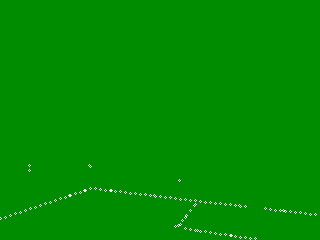
\includegraphics[width=0.3\textwidth]{figures/points.png}
\end{figure}

Once these points have generated, the next step is to connect them in order to form line segments. For the representation of each line segment we hold a queue of points, at each time the line segment is formed by the first and the last point in the queue as starting and ending points. Pushing always the first point of the vector in the queue and deleting it from the vector the same time, we are looking for the closest points (5 points) to this point. From these closest points, we are checking the white ratio between these points and our initial point. Assuming that points from the same line segment, do not have black pixels between them, we connect the closest one with high white ratio, usually $1.0$, and pushing it in the queue of points as the last element and deleting it from the vector. The same procedure continues, but now we are looking to connect the last element on the queue with one from the remaining points in this vector. So, now the question is how are we going to stop connecting points? Considering a line formed by a many points, these points have to have small distance from the projection point on the line. Based on this idea, we can introduce an error function in order to define when a line starts not to comply with the points consisting it. Assuming a queue of points $Q$, which stores $n$-points, we can say that:
\begin{equation}
Error_Q = \sum_{i=1}^{n}(Eucl.Dist(Q_i, Proj.Point(Q_i,Q)))^2
\end{equation}
This error measure proved to be really informative in our case to understand when a line is starting to consist of points which may not represent the same line segment. When this error becomes larger than a threshold, we store the produced line so far, and we continue with the next point in the vector. To store the line, we first check if there is an already stored line which is an extension of the current line, to find out we measure the error we introduced in equation 1, taking now as line's starting and ending points the points with the largest distance between them. If the error remains small enough, and the closest points of this connection are covered in high white ratio, then we merge these lines which now represent a continuous line. 
\begin{algorithm}[t!]
\caption{Line segment detection algorithm}
\label{line}
\begin{algorithmic}[1]
\STATE {\bf Input: }$points, image$
\STATE {\bf Output: }$line$
\STATE{start = points[0]}
\WHILE{points.size() $\neq$ 0}
\STATE{line.push(start)}
\STATE{bestCandidate = findBestCandidate(points, image)}
\STATE{points.erase(bestCandidate)}
\STATE{error = computeError(line, bestCandidate)}
\IF{error < threshold}
\STATE{start = bestCandidate}
\ELSE
\STATE{storeLine(line)}
\STATE{line.clear()}
\ENDIF
\ENDWHILE
\end{algorithmic}
\end{algorithm}
Algorithm~\ref{line}, presents the pseudo-code for the line detection procedure. In line $12$, function $storeLine$, takes as input the produced line, if the line cannot be merged with an already stored line segment, then, it is stored as it is in a vector of lines.






\end{document}